% !TEX program = xelatex
% !BIB program = biber
% !TEX options = -synctex=1 -file-line-error -halt-on-error -xelatex -shell-escape "%DOC%"
\documentclass[10pt,aspectratio=1610,table]{beamer}
\usepackage{hyperref} % Create hyperlinks in your document
% Use author-title-year bibstyle, copied from:
% https://tex.stackexchange.com/questions/249762/biblatex-verbose-style-adding-year-to-the-author-title-format
\usepackage[backend=bibtex, bibstyle=authoryear, citestyle=verbose-trad1, indexing=cite, giveninits=true, citepages=omit]{biblatex}
\newbibmacro*{cite:labeldate+extradate}{%
  \iffieldundef{labelyear}
    {}
    {\printtext[parens]{%
        \printtext[bibhyperref]{%
          \printlabeldateextra}}}}

  \renewbibmacro*{cite:name}{%
    \printnames{labelname}%
    \setunit{\printdelim{nameyeardelim}}%
    \usebibmacro{cite:labeldate+extradate}%
    \setunit*{\printdelim{nametitledelim}}}

  \renewbibmacro*{cite:idem}{%
    \bibstring[\mkibid]{idem\thefield{gender}}%
    \setunit{\printdelim{nameyeardelim}}%
    \usebibmacro{cite:labeldate+extradate}%
    \setunit{\printdelim{nametitledelim}}}
% \renewcommand*{\bibfont}{\tiny}
\addbibresource{bibliography.bib}
%\usepackage{newtxmath} % Use New TX font for math
%\usepackage{stix2} % Use stix2 font for math
\usepackage[no-math]{fontspec}
\usepackage{xeCJK} % Chinese font setting
\usepackage{tcolorbox} % Coloured boxes, for LATEX examples and theorems, etc
\tcbuselibrary{skins, breakable, theorems}
\usepackage{url} % Inserting urls
\usepackage{caption} % Customising captions in floating environments
\usepackage{verbatim}
\usepackage{multicol} % Multi-columns
\usepackage{multirow} % Multi-rows
\usepackage{booktabs} % Better tables
\usepackage{tikz} % For plot
\usepackage{pgf-pie} % For plotting pie chart
\usetikzlibrary{angles, arrows.meta, quotes, calc, intersections}
\usepackage{pgfplots}
\pgfplotsset{compat=1.16}
\usepackage{soul} % For smallcaps/striking out/highlighting
\sethlcolor{cuhklightyellow}
\usepackage{listings} % For source code
\usepackage{minted} % For source code
\usepackage{sourcecodepro} % For using source code pro as the default typewriter font
\usepackage{ifplatform} % For identifying OS platforms
\usepackage[vlined, ruled, linesnumbered]{algorithm2e} % For algorithms
\usepackage{algorithmic}
\usepackage{amsmath} % For math symbols
\usepackage{amssymb}
\usepackage{stmaryrd}
\usepackage{pifont}
\usepackage{varwidth}
\usepackage{braket} % For quantum Dirac notation
\usepackage{derivative} % For derivatives
\usepackage{microtype} % For typographical perfection

% Some packages and configurations for math
\usepackage{bm}
\renewcommand{\vec}[1]{\bm{#1}}
\DeclareMathOperator*{\E}{\mathbb{E}}
\DeclareMathOperator*{\Var}{\mathrm{Var}}
\DeclareMathOperator*{\Cov}{\mathrm{Cov}}
\DeclareMathOperator*{\argmin}{\mathrm{arg\,min\;}}
\DeclareMathOperator*{\argmax}{\mathrm{arg\,max\;}}
\def\ZZ{{\mathbb Z}}
\def\NN{{\mathbb N}}
\def\RR{{\mathbb R}}
\def\CC{{\mathbb C}}
\def\QQ{{\mathbb Q}}
\def\FF{{\mathbb F}}
\def\EE{{\mathbb E}}
\newcommand{\tr}{{\rm tr}}
\newcommand{\sign}{{\rm sign}}
\usepackage{bbm}
\usepackage{physics}
\let\div\divisionsymbol
\usepackage{blkarray}
\newcommand{\1}{\mathbbm{1}}
\newcommand{\inprod}[2]{\left\langle #1, #2 \right\rangle}
% \newcommand{\set}[1]{\left\{#1\right\}}

% Set minted style and font size, used for displaying source code
\setminted{frame=lines, breaklines, xleftmargin=16pt, linenos, fontsize=\fontsize{7}{7}, style=friendly, baselinestretch=1.2}

% For inline code, use the current font size
\makeatletter
\newcommand{\currentfontsize}{\fontsize{\f@size}{\f@baselineskip}\selectfont}
\makeatother
\setmintedinline{fontsize=\currentfontsize}

% Define CUHK theme colors
\definecolor{cuhkpurple}{RGB}{117,15,109}
\definecolor{cuhkyellow}{RGB}{221,163,0}
\definecolor{cuhkblackyellow}{RGB}{153,102,0}
\definecolor{cuhklightyellow}{RGB}{244,223,176}

% Define Theorem box style
\newtcbtheorem{theo}{Theorem}%
  {enhanced, breakable,
    colback = white, colframe = cuhkpurple, colbacktitle = cuhkpurple,
    attach boxed title to top left = {yshift = -2mm, xshift = 5mm},
    boxed title style = {sharp corners},
    fonttitle = \sffamily\bfseries}{th}

% Define Chinese fonts 
\setCJKmainfont{Noto Sans CJK TC}
\setCJKsansfont{Noto Sans CJK TC}
\setCJKmonofont{Noto Sans Mono CJK TC}

% Define English fonts 
\usefonttheme{professionalfonts}
\setmainfont[Mapping=tex-text]{Lato}
\setsansfont{Lato}
\setmonofont{Source Code Pro}

% Template theme
\useoutertheme{infolines}
\setbeamertemplate{navigation symbols}{}
\usetheme[height=10mm]{Rochester}
\usecolortheme[named=cuhkpurple]{structure}
\setbeamercolor{block title example}{use=structure,fg=white, bg=cuhkyellow}
\setbeamercolor{block body example}{use=structure,fg=black, bg=cuhklightyellow}
\setbeamercolor{alerted text}{fg=cuhkpurple, bg=cuhklightyellow}
\setbeamercolor{frametitle}{fg=white, bg=cuhkpurple}

% Some useful definitions
\newcommand{\boxalert}[1]{{
    \usebeamercolor{alerted text}\colorbox{bg}{\alert{#1}}
}}

\newcommand{\cmark}{\ding{51}}
\newcommand{\xmark}{\ding{55}}

%% Logo
\titlegraphic{
    \includegraphics[width=4cm]{The-Chinese-University-of-Hong-Hong-logo.eps}
}



\title[Sample]{CUHK Beamer Template}
\subtitle{Sample Slides}
\author[Li Zhuohua]{Li Zhuohua}
\institute[CUHK]{The Chinese University of Hong Kong}
\date{\today}

\begin{document}

\frame[plain]{\maketitle}

%\begin{frame}{Outline}
%  \tableofcontents{}
%\end{frame}

\begin{frame}{Itemize Tests}
	\renewcommand{\outlineii}{enumerate}
	\begin{outline}
		\1 One: \textit{Two} \textbf{Three}
			\2 \so{letterspacing}
			\2 \ul{underlining}
			\2 \st{striking out}
			\2 \hl{highlighting}
			\2 \caps{CAPITALS, Small Capitals}
		\1 Test Test Test
	\end{outline}
\end{frame}

\begin{frame}{Multi-Columns}
	\begin{multicols}{3}
    [
    All human things are subject to decay. And when fate summons, Monarchs must obey.
    ]
    Hello, here is some text without a meaning.  This text should show what 
    a printed text will look like at this place.
    If you read this text, you will get no information.  Really?  Is there 
    no information?  Is there...
    \end{multicols}
\end{frame}

\begin{frame}{Plot Test}
    \pgfplotsset{width=5.5cm,compat=1.9}
    \begin{figure}
        \centering
        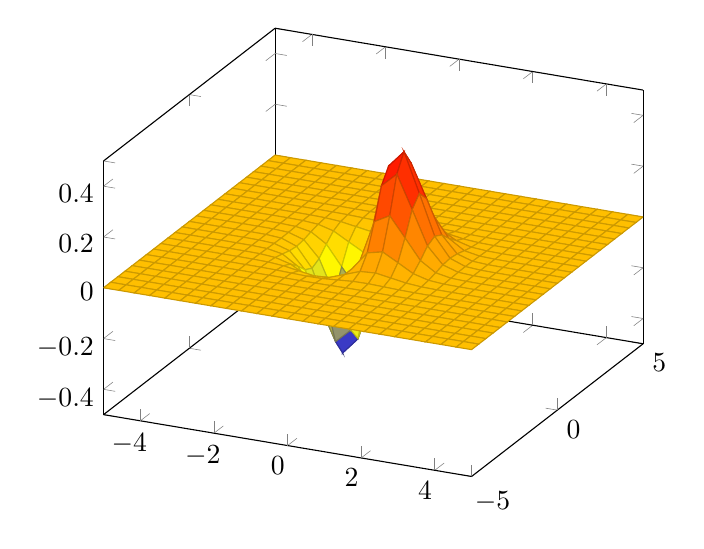
\begin{tikzpicture}
            \begin{axis}
                \addplot3[
                surf,
                ]
                {exp(-x^2-y^2)*x};
            \end{axis}
        \end{tikzpicture}
        \caption{Plot $z=x(-x^2-y^2)$} \label{fig:plot}
    \end{figure}
\end{frame}

\begin{frame}{中文测试中文測試}
	\begin{outline}
		\1 这是简体中文這是繁體中文: \textbf{加粗} + \underline{下划线下劃線} + \textit{斜体斜體}
			\2 这是第二层
			\2 這是第二層
	\end{outline}
\end{frame}

\begin{frame}{Citation Tests}
	\begin{outline}
		\1 Yao's Millionaires' problem~\footcite{10.5555/1382436.1382751}
	\end{outline}
\end{frame}

\begin{frame}{Algorithm Test}
    \IncMargin{1em}
    \begin{algorithm}[H]
      \DontPrintSemicolon
      \SetVlineSkip{0pt}
      \scriptsize
      \SetKwFunction{Successors}{\textsc{Successors}}%
      \SetKwFunction{Entry}{\textsc{Entry}}%
      \SetKwFunction{Transfer}{\textsc{Transfer}}%
      \KwIn{Control Flow Graph: $CFG$}%
      \KwOut{Invariant: $State$}%
      initialization: \parbox[t]{\linewidth}{
        $State[n] \leftarrow \top$ if $n=\Entry{CFG}$\;
        $State[n] \leftarrow \bot$ otherwise\;}
    
      $WorkList \leftarrow \Entry{CFG}$\;
      \While{$WorkList$ is not empty}{
        $WorkList \leftarrow WorkList \backslash \{n\}$\;
        $new\_state \leftarrow \Transfer{State[n]}$\;
        \ForEach{$succ \in \Successors{CFG, n}$} {
          \If{$new\_state \not\sqsubseteq State[succ]$} {
            $State[succ] \leftarrow State[succ] \sqcup new\_state$\;
            $WorkList \leftarrow WorkList \cup \{succ\}$\;
          }
        }
      }
      \SetAlCapHSkip{.5em}
      \caption{Basic algorithm for Abstract Interpretation}
    \end{algorithm}
\end{frame}

\begin{frame}[fragile]{Code Test}
    \begin{minted}{rust}
fn main() {
    println!("Hello World!");
}
    \end{minted}
	\begin{outline}
		\1 Inline code is also supported: \mintinline{rust}{fn main() { }}
	\end{outline}
\end{frame}

\begin{frame}{Math Test}
    \begin{enumerate}
        \item Symbols: $\alpha,\beta,\gamma,\delta,\epsilon,\varepsilon,\zeta,\eta,\theta,\vartheta,\iota,\kappa,\lambda,\nu,\xi,\varpi,\rho,\varrho,\sigma,\varsigma,\tau,\upsilon,\phi,\varphi,\chi,\psi,\omega$;
        \item Symbols: $f'',\sqrt{a},\overrightarrow{a},\subseteq,\supseteq$
        \[\int,\iint,\iiint,\iiiint,\oint\]
        \item Complex equation:
        \resizebox{.9\hsize}{!}{%
        $
        \displaystyle\lim_{x\rightarrow 0^+}\displaystyle\lim_{y\rightarrow +\infty}\frac{\displaystyle\sum_{n=1}^{\infty}{\frac{\left(-1\right)^{n-1}}{n}}\displaystyle\sum_{m=0}^{\infty}{\frac{1}{n2^m+1}}\displaystyle\int_0^{x^2}{\frac{\pi \left(\sqrt[4]{1+t}-1\right)\sin t^4}{\displaystyle\sum_{n=1}^{\infty}{\displaystyle\frac{\left(\left(n-1\right)!\right)^2\left(2t\right)^{2n}}{\left(2n\right)!}}\displaystyle\int_0^1{\displaystyle\frac{\left(1-2x\right)\ln\left(1-x\right)}{x^2-x+1}\textrm{d}x}}\textrm{d}x}}{x^2\left(x-\tan x\right)\ln\left(x^2+1\right)\left[\left(\displaystyle\frac{2\arctan\frac{y}{x}}{\pi}\right)^y-1\right]}=\frac{27}{32}
        $
        }
    \end{enumerate}
\end{frame}

\begin{frame}{Theorem/Lemma/Corollary/Proof}
    Fancy style theorem:
	\begin{theo}{Pythagorean Theorem}{pythagoras}
		For a right triangle with legs $a$ and $b$ and hypotenuse $c$,
		\[
		a^2 + b^2 = c^2. 
		\]
	\end{theo}
	This is a reference to Theorem \ref{th:pythagoras}.
    
    Normal style theorem:
    \begin{theorem}[Fixed-point Theorem]
        In a lattice $L$ with finite height, every monotone function $f : L \rightarrow L$
        has a unique least fixed-point denoted $fix (f)$ defined as:
        \[
        fix (f) = \bigsqcup_{i \geq 0}f^i(\bot)
        \]
    \end{theorem}
\end{frame}

\begin{frame}{Theorem/Lemma/Corollary/Proof}
    \begin{lemma}[Lemma Name]
        $ x + y = y + x  $
    \end{lemma}
    
    \begin{corollary}[Corollary Name]
        There's no right rectangle whose sides measure 3cm, 4cm, and 6cm.
    \end{corollary}
    
    \begin{proof}[\proofname\ (Theorem \ref{th:pythagoras})]
        $\omega +\phi = \epsilon $
    \end{proof}
\end{frame}

\setbeamertemplate{headline}{}
\addtobeamertemplate{frametitle}{\vspace*{-0.9\baselineskip}}{}
\begin{frame}{}
    \centering \Huge
    \emph{Thank You}
\end{frame}

\begin{frame}[allowframebreaks]
    References
	\printbibliography
\end{frame}

\end{document}